\begin{tikzpicture}

\GraphInit[vstyle=Classic]

\Vertex[Lpos=90, x=0, y=0, L=$U$]{U};
\Vertex[Lpos=-90, x=0, y=0, L=$u$]{u};
\Vertex[Lpos=90, x=2, y=0, L=$X$]{X};
\Vertex[Lpos=-90, x=2, y=0, L=$x$]{x};
\Vertex[Lpos=90, x=4, y=0, L=$Y$]{Y};
\Vertex[Lpos=-90, x=4, y=0, L=$y$]{y};
\Vertex[Lpos=90, x=6, y=0, L=$Z$]{Z};
\Vertex[Lpos=-90, x=6, y=0, L=$b$]{b};
\Vertex[Lpos=90, x=8, y=0, L=$W$]{W};
\Vertex[Lpos=-90, x=8, y=0, L=$d$]{d};
\Vertex[empty, x=10, y=0]{O};

\Edge[style ={-}, label={$UX$}, labelstyle={above}]({U})({X})
\Edge[style ={draw=none}, label={$p$}, labelstyle={below}]({U})({X})
\Edge[style ={-}, label={$XY$}, labelstyle={above}]({X})({Y})
\Edge[style ={draw=none}, label={$q$}, labelstyle={below}]({X})({Y})
\Edge[style ={-}, label={$YZ$}, labelstyle={above}]({Y})({Z})
\Edge[style ={draw=none}, label={$a$}, labelstyle={below}]({Y})({Z})
\Edge[style ={-}, label={$ZW$}, labelstyle={above}]({Z})({W})
\Edge[style ={draw=none}, label={$c$}, labelstyle={below}]({Z})({W})
\Edge[style ={-}, label={}]({W})({O})

\end{tikzpicture}
